\section{Lecture 3 -- 8th November 2024}\label{sec: lecture 3}
Let situate our discussion of the phenomena encountered in \Cref{sec: lecture 2} in a larger context, with an eye towards discussing the observations made here more rigorously over the rest of the semester.

Recall that per \Cref{prop: asymptotics q t Pochhammer at 1} that the asymptotics of the $q$-Pochhammer $(t;q)_{\infty}$ at $q\to 1$ is given by 
$$\exp\left(\frac{\Li_{2}(t)}{h}\right)\cdot\sqrt{1-t}\cdot O(h)$$
where $O(h)\in\QQ[t,\frac{1}{1-t}][[h]]$. Note that the $q$-Pochhammer naturally admits an expansion in the ring $\QQ[[t]]((h))$ of power series in $t$ and Laurent series in $h$. Thus, dividing by the exponential prefactor, we would expect the ratio 
$$\frac{(t;q)_{\infty}}{\exp\left(\frac{\Li_{2}(t)}{h}\right)\sqrt{1-t^{2}}}$$
to lie in $\QQ[t,\frac{1}{1-t}][[h]]\subseteq\QQ[[t,h]]$ as well. Similarly following \Cref{prop: asymptotics of q t Pochhammer at root of unity}, we expect the ratio 
$$\frac{(t;q)_{\infty}}{\exp\left(\frac{\Li_{2}(t^{m})}{m^{2}h}\right)\frac{\sqrt{1-t^{m}}}{\prod_{i=0}^{m-1}(1-\zeta_{m}^{i}t)^{i/m}}}$$
to lie in $\QQ(\zeta_{m})[t,\frac{1}{1-t^{m}}][[h]]$ as $q\to\zeta_{m}$. It is especially surprising that these expansions have good algebraicity properties in the variable $t$.  

Moreover, these power series $O(h)$ appearing above have good $p$-adic properties, giving arithmetic meaning to the expansions of $(t;q)_{\infty}$ with the $\Li_{2}$ term of the abovementioned equations giving the Borel regulator on the third algebraic $K$-group, and the term $\prod_{i=0}^{m-1}(1-\zeta_{m}^{i}t)$ of the latter equation the modulo $m$ \'{e}tale regulator of the third algebraic $K$-group. 

This peculiar behavior of such power series was first observed by Garoufalidis and Zagier who showed that for a Nahm sum $f_{A}(q)$ with associated number field $\KK$
$$f_{A}(q)\sim\exp(\Li_{2}(\xi))\cdot\frac{\sqrt{\delta}}{\sqrt[m]{\varepsilon_{m}(\xi)}}\cdot O(h)$$
for some class $\xi\in K_{3}(\KK)$ and $O(h)\in\KK(\zeta_{m})[[h]]$ as $q\to\zeta_{m}$. Writing $O(h)$ as $g_{A,m}$ and consider 
$$g_{A,m}\in \frac{\sqrt{\delta}}{\sqrt[m]{\varepsilon_{m}(\xi)}}\cdot\KK(\zeta_{m})[[h]]\cong\frac{\sqrt{\delta}}{\sqrt[m]{\varepsilon_{m}(\xi)}}\cdot\KK(\zeta_{m})[[q-\zeta_{m}]]$$
under the identification $q=\zeta_{m}\exp(h)$ where $\delta,\varepsilon_{m}(\xi)$ are transcendental. 
\begin{remark}
    It is unclear if $\delta$ is a function of $\xi$. 
\end{remark}
\begin{remark}
    These $g_{A,m}$ have huge coefficients -- slightly worse than factorial where the degree $p-2$ coefficients have $p$ in the denominator. 
\end{remark}
One then hopes that to each $g_{A,m}$ and a class $\xi\in K_{3}(\KK)$ one can associate a power series 
$$g_{m}(\xi)\in\frac{\sqrt{\delta}}{\sqrt[m]{\varepsilon_{m}(\xi)}}\cdot\KK_{p}^{\wedge}(\zeta_{m})[[q-\zeta_{m}]]$$
with $\KK_{p}^{\wedge}$ the $p$-adic completion of $\KK$ such that the ratio $g_{A,m}/g_{m}(\xi)$ has $p$-integral coefficients. 

While it is yet uncear how to realize this on the nose, the product 
\begin{equation}\label{eqn: symmetrization}
    h_{A,m}(q)=g_{A,m}(q)g_{A,m}(q^{-1})\in\Ocal_{\KK}\left[\zeta_{m},\frac{1}{\Delta}\right][[q-\zeta_{m}]]
\end{equation}
cancels out the preceding transcendental terms and where $\Delta$ is the discriminant of the number field $\KK$. 

The $p$-adic properties can be studied in an appropriate generalization of the Habiro ring, but the case of the (ungeneralized) Habiro ring as in \Cref{def: Habiro ring} is already interesting. 
\begin{proposition}\label{prop: isomorphism of Habiro ring}
    Let $\Hcal$ be the Habiro ring. There is an isomorphism 
    $$\Hcal\cong\left\{(h_{m})_{m\geq 1}:\substack{h_{m}\in\ZZ[\zeta_{m}][[q-\zeta_{m}]] \text{ such that for all primes }p\\ h_{m}=h_{pm}\in\ZZ_{p}[\zeta_{m}][[q-\zeta_{m}]]\cong\ZZ_{p}[\zeta_{pm}][[q-\zeta_{pm}]]}\right\}.$$
\end{proposition}

\begin{figure}[H]
    \tikzset{every picture/.style={line width=0.75pt}} %set default line width to 0.75pt        

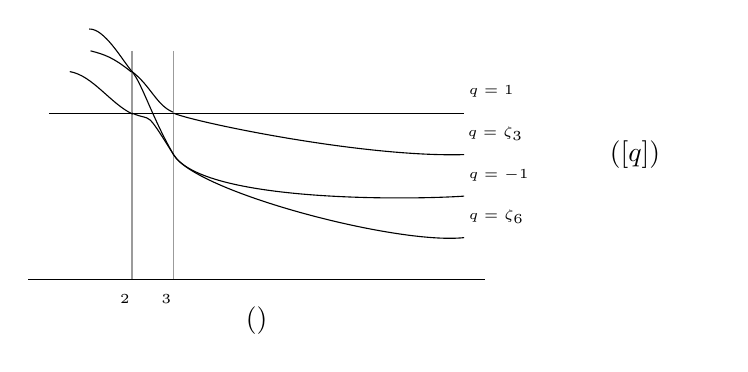
\begin{tikzpicture}[x=0.75pt,y=0.75pt,yscale=-1,xscale=1]
%uncomment if require: \path (0,300); %set diagram left start at 0, and has height of 300

%Straight Lines [id:da5858698884102702] 
\draw    (40,180) -- (260,180) ;
%Straight Lines [id:da23025189850916727] 
\draw [color={rgb, 255:red, 155; green, 155; blue, 155 }  ,draw opacity=1 ]   (90,70) -- (90,180) ;
%Straight Lines [id:da687814768445594] 
\draw [color={rgb, 255:red, 155; green, 155; blue, 155 }  ,draw opacity=1 ]   (110,70) -- (110,180) ;
%Straight Lines [id:da16720674157357007] 
\draw    (50,100) -- (250,100) ;
%Curve Lines [id:da427587550617629] 
\draw    (70,70) .. controls (76.77,71.74) and (81,73.17) .. (89.67,80.17)(90,80) .. controls (99,86.83) and (101.66,96.05) .. (109.69,99.55)(110,100) .. controls (118.34,103.95) and (200.31,121.38) .. (250,120) ;
%Curve Lines [id:da03299723689278511] 
\draw    (60,80) .. controls (71,81.83) and (79.67,95.5) .. (90.33,100.5)(90,100) .. controls (100.33,104.5) and (95.67,97.17) .. (110.33,120.5)(110,120) .. controls (124.33,142.83) and (222.66,141.88) .. (250,140) ;
%Curve Lines [id:da04335961004381472] 
\draw    (69.33,59.5) .. controls (76.66,59.11) and (85.04,74.09) .. (90,80) .. controls (94.96,85.91) and (99.67,102.17) .. (110,120) .. controls (120.33,137.83) and (217,163.5) .. (250,160) ;

% Text Node
\draw (150,200) node   [align=left] {\begin{minipage}[lt]{54.4pt}\setlength\topsep{0pt}
\begin{center}
$\spec(\ZZ)$
\end{center}

\end{minipage}};
% Text Node
\draw (90,190) node   [align=left] {\begin{minipage}[lt]{8.67pt}\setlength\topsep{0pt}
{\tiny $\displaystyle 2$}
\end{minipage}};
% Text Node
\draw (270,110) node   [align=left] {\begin{minipage}[lt]{27.2pt}\setlength\topsep{0pt}
{\tiny $\displaystyle q=\zeta _{3}$}
\end{minipage}};
% Text Node
\draw (275,150) node   [align=left] {\begin{minipage}[lt]{34pt}\setlength\topsep{0pt}
{\tiny $\displaystyle q=\zeta _{6}$}
\end{minipage}};
% Text Node
\draw (110,190) node   [align=left] {\begin{minipage}[lt]{8.67pt}\setlength\topsep{0pt}
{\tiny $\displaystyle 3$}
\end{minipage}};
% Text Node
\draw (275,90) node   [align=left] {\begin{minipage}[lt]{34pt}\setlength\topsep{0pt}
{\tiny $\displaystyle q=1$}
\end{minipage}};
% Text Node
\draw (275,130) node   [align=left] {\begin{minipage}[lt]{34pt}\setlength\topsep{0pt}
{\tiny $\displaystyle q=-1$}
\end{minipage}};
% Text Node
\draw (332.33,120) node   [align=left] {\begin{minipage}[lt]{54.4pt}\setlength\topsep{0pt}
\begin{center}
$\spec(\ZZ[q])$
\end{center}

\end{minipage}};


\end{tikzpicture}

\caption{$p$-adic behavior of Habiro ring elements.}
\end{figure}
\begin{corollary}\label{corr: injection to power series in q minus 1}
    There is an injection $\Hcal\hookrightarrow\ZZ[[q-1]]$. 
\end{corollary}
\begin{corollary}\label{corr: injection to product of adjointing roots of unity}
    The map $\Hcal\to\prod_{m\geq 1}\ZZ[\zeta_{m}]$ by $h\mapsto (h(\zeta_{m}))_{m}$ is injective. 
\end{corollary}
This behavior suggests that the Habiro ring is much more structured than a ring of functions that admits asymptotic expansions at all roots of unity, and is in this sense quite rigid. This is observed, for example, in the $p$-adic ``coherence'' behavior of the series appearing in the description of \Cref{prop: isomorphism of Habiro ring}.

Unfortunately, this na\"{i}ve definition of the Habiro ring cannot be nicely generalized. Garoufalidis and Zagier observed that for $h_{A,m}\in\Ocal_{\KK}\left[\zeta_{m},\frac{1}{\Delta}\right][[q-\zeta_{m}]]$, it is not the case that $h_{A,m}$ agrees with $h_{A,pm}$ as elements of $\Ocal_{\KK_{p}^{\wedge}}\left[\zeta_{m},\frac{1}{\Delta}\right][[q-\zeta_{m}]]$, though it does agree up a sign depending on the residue class of the prime $p$ modulo 3 in a special case, suggesting that compatibility could indeed be defined. This allows us to give the eponymous definition. 
\begin{definition}[Habiro Ring of a Number Field]\label{def: Habiro ring of a number field}
    Let $\KK$ be a number field with discriminant $\Delta$. The Habiro ring of $\KK$ is given by 
    $$\Hcal_{\Ocal_{\KK}[\frac{1}{\Delta}]}=\left\{(h_{m})_{m\geq1}:\substack{h_{m}\in\Ocal_{\KK}[\zeta_{m},\frac{1}{\Delta}][[q-\zeta_{m}]] \\
    \forall p\nmid\Delta, h_{m}=\varphi_{p}(h_{pm})\in(\Ocal_{\KK})_{p}^{\wedge}[\zeta_{m},\frac{1}{\Delta}][[q-\zeta_{m}]]}\right\}$$
    where $(\Ocal_{\KK})_{p}^{\wedge}$ is the $p$-adic completion of $\Ocal_{\KK}$ and $\varphi_{p}$ the Frobenius lift on $(\Ocal_{\KK})_{p}^{\wedge}$. 
\end{definition}
\begin{remark}
    $(\Ocal_{\KK})_{p}^{\wedge}$ is a finite \'{e}tale $\ZZ_{p}$-algebra, and the Frobenius lifts uniquely to an endomorphism on the $p$-adic completion. \'{E}taleness of the $\ZZ_{p}$-algebra explains uniqueness of the Frobenius.  
\end{remark}
While this definition is the appropriate generealization of the Habiro ring, it is yet unclear how explicit elements of this ring can be constructed. In fact, there is no map in general $\Ocal_{\KK}\to\Hcal_{\Ocal_{\KK}[\frac{1}{\Delta}]}$ -- the constant map to power series does not satisfy the identity on the Frobenius lift. 
\begin{remark}
    In special cases, such as $\KK/\QQ$ being an Abelian extension, an ad-hoc construction for a map can be made. 
\end{remark}
This behavior is analogous to the nice behavior of the ``symmetrization'' of (\ref{eqn: symmetrization}), and we thus expect that for each $\xi\in K_{3}(\KK)$ there is a unique (up to unique isomorphism) locally free rank 1 module or line bundle $L(\xi)$ over $\Hcal_{\Ocal_{\KK}[\frac{1}{\Delta}]}$ (resp. $\spec(\Hcal_{\Ocal_{\KK}[\frac{1}{\Delta}]}))$ which naturally contains $(g_{A,m})_{m}$, the power series of asymptotic expansions at roots of unity, as an element (resp. section). In fact, if two matrices $A_{1},A_{2}$ define the same number field $\KK$ and $\xi\in K_{3}(\KK)$ as in the procedure of (\ref{eqn: number field of Nahm equation}), then the ratios of the asymptotic expansions at roots of unity
$$\left(\frac{g_{A_{1},m}}{g_{A_{2},m}}\right)\in\mathrm{Frac}\left(\Hcal_{\Ocal_{\KK}[\frac{1}{\Delta}]}\right)$$
which produces a natural map $K_{3}(\KK)\to\sfPic(\Hcal_{\Ocal_{\KK}[\frac{1}{\Delta}]})$ to the Picard groupoid of line bundles/invertible modules over the Habiro ring of the number field. 

As we will soon see, all the expectations above hold, and will be made precise in what follows. 